\setchapterpreamble[u]{\margintoc}
\chapter{Distribuzione e gestione delle chiavi crittografiche}
\labch{chapter3}

La sicurezza delle chiavi crittografiche dipende dal modo con cui sono protette. Il managment di queste chiavi comprende la loro generazione, creazione, protezione, salvataggio, scambio, sostituzione e uso. Permette inoltre di restringere l'accesso alle chiavi e monitorarne/registrarne ogni accesso, uso e contesto.
Il sistema di gestione delle chiavi comprende anche le chiavi dei server, le procedure utente e i protocolli.
La sicurezza del sistema crittografico dipende anche da una gestione corretta delle chiavi.

Tecnica di distribuzione delle chiavi: 
\begin{itemize}
    \item Riguarda la consegna di una chiave a due parti che vogliono scambiarsi dati senza che terzi vedano la chiave;
	\item Affichè la crittografia simmetrica funziona, le due parti devono condividere la stessa chiave, che deve essere protetta da accessi non autorizzati;
	\item È desiderabile cambiare frequentemente la chiave per limitare la quantità di dati che verrebbero compromessi se un attaccante ottenesse la chiave.
\end{itemize}

Possibili modi per la distribuzione di chiavi simmetriche (figura \ref{fig:3-1}):
\begin{itemize}
    \item A sceglie una chiave e la consegna fisicamente a B;
	\item Un terzo sceglie la chiave e la consegna fisicamente ad A e B;
	\item Se A e B hanno condiviso una chiave recentemente, un terzo può scegliere una nuova chiave e inviarla, cifrata con la vecchia chiave, ad A e B;
    \item Se A e B hanno una connessione cifrata con C, C può inviare la chiave sul canale cifrato ad A e B.
\end{itemize}

In riferimento allo schema:
\begin{itemize}
    \item Key Transaltion Center: riceve una chiave da un'entità A cifrata con una chiave simmetrica condivisa tra A e KTC, la decifra e la invia all'entità B cifrata con la chiave simmetrica condivisa tra B e KTC. È considerato trusted.
    \item Kma: chiave simmetrica condivisa tra A e KTC. Esiste quindi un canale sicuro tra i due.
\end{itemize}

\begin{figure}
    \centering
    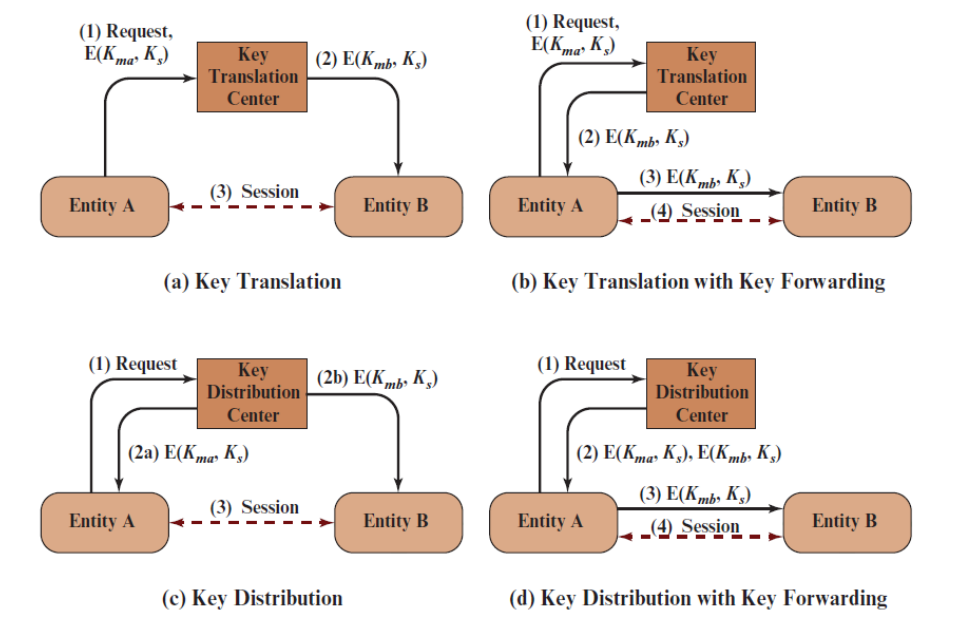
\includegraphics[width=1\textwidth]{images/chapter3/3-1.png}
    \caption{Possibili distribuzioni della chiave.}
    \label{fig:3-1}
\end{figure}

Generalmente la chiave simmetrica scambiata all'inizio della comunicazione viene considerata come master key e usata per generare una serie di sottochiavi simmetriche. Più in basso nella gerarchia sono le sottochiavi, più la loro durata diminuisce e il loro uso aumenta.

\paragraph{Semplice scambio di chiavi usando chiavi pubbliche} A invia la propria chiave pubblica e identità a B. B risponde inviando la chiave di sessione cifrata con la chiave pubblica di A (figura \ref{fig:3-2}). 

\begin{figure}
    \centering
    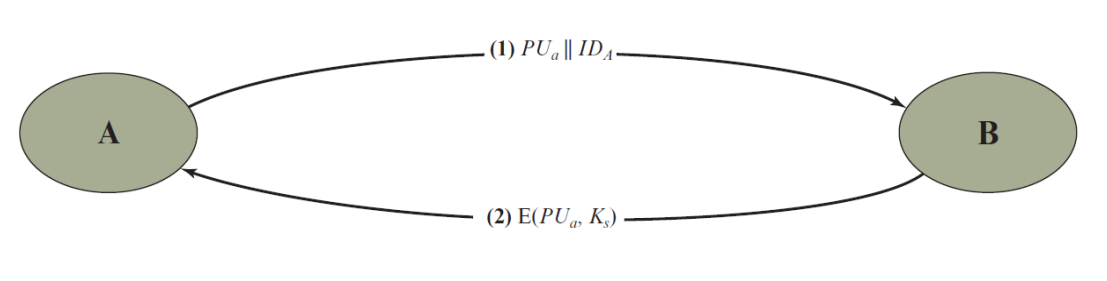
\includegraphics[width=1\textwidth]{images/chapter3/3-2.png}
    \caption{Scambio semplice.}
    \label{fig:3-2}
\end{figure}

Questa soluzione è però debole ad un attacco man-in-the-middle: 
\begin{enumerate}
    \item C cattura il messaggio di A; 
	\item Sostituisce la chiave pubblica di A con la sua (lasciando inalterata l'identità);
	\item B codifica la chiave di sessione con la PU che crede sia di A e invia il messaggio;
	\item C cattura la risposta, decifra il messaggio, lo ricifra con la PU di A e glielo invia;
	\item A riceve la chiave e la comunicazione è stabilità;
	\item C può decifrare ora tutti i messaggi scambiati sul canale.
\end{enumerate}

\paragraph{Scambio di chiavi con chiavi pubbliche e nonce\sidenote{Nonce: stringa randomica che viene usata per verificare che un messaggio non sia stato modificato/sostituito (protegge anche dai replay attack). Se la risposta non contiene lo stesso nonce che ho inviato nella richiesta, allora la scarto.}} Lo scambio prevede una serie di passaggi (figura \ref{fig:3-3}):
\begin{itemize}
    \item A invia la propria identità e un nonce entrmbi cifrati con la PU di B; 
    \item B Invia il nonce generato da A e un proprio nonce cifrati con la PU di A;
    \item A invia il nonce ricevuto da B cifrato con la PU di B;
    \item A e B si sono ora autenticati l'un l'altro, quindi B invia la chiave di sessione cifrata con la propria chiave privata, il tutto cifrato con la chiave pubblica di B.
\end{itemize}

\begin{figure}
    \centering
    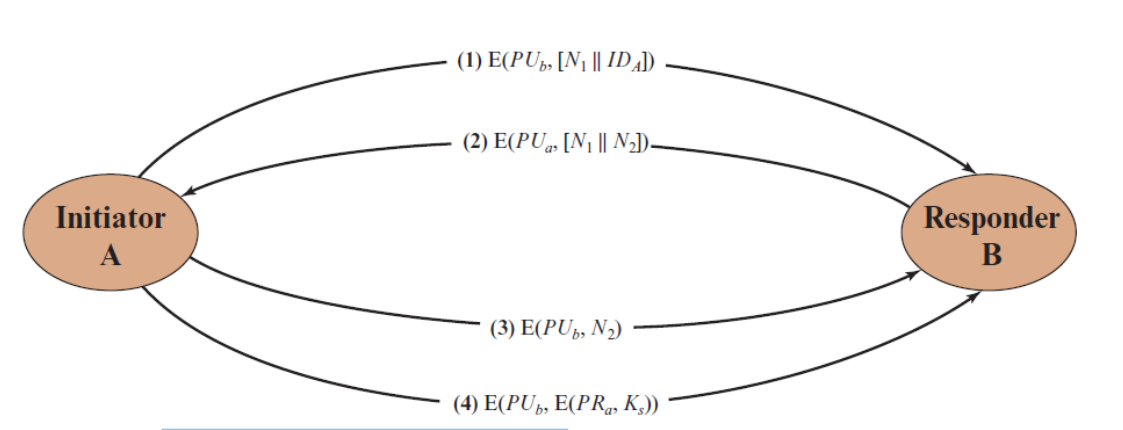
\includegraphics[width=1\textwidth]{images/chapter3/3-3.png}
    \caption{Scambio semplice.}
    \label{fig:3-3}
\end{figure}

Anche questo scambio è debole, in quanto C può mettersi in mezzo e far credere ad A e B, nei primi 3 passi, di star comunicando.

\section{Distribuzione delle chiavi pubbliche}

L'autority mantiene una directory con nome/certificato,chiave pubblica, che è facilmente accessibile.

Scenario di distribuzione (figura \ref{fig:3-4}):
\begin{enumerate}
    \item A richiede all'autority la chiave pubblica di B. Nel messaggio inserisce un timestamp;
	\item L'autority invia la chiave cifrata con la chiave pubblica dell'autority. Nel messaggio cifrato riporta il timestamp ricevuto da A;
	\item A invia la propria identità e un nonce a B;
	\item B richiede all'authority la chiave pubblica di A. Nel messaggio inserisce un timestamp;
	\item L'autority invia la chiave pubblica di A cifrata con la chiave privata dell'autority. Nel messaggio cifra anche il timestamp ricevuto;
	\item B invia, cifrati con la chiave pubblica di A, il nonce ricevuto da A e un nonce da lei generato;
	\item A invia a B il nonce ricevuto cifrato con la chiave pubblica di B.
\end{enumerate}

\begin{figure}
    \centering
    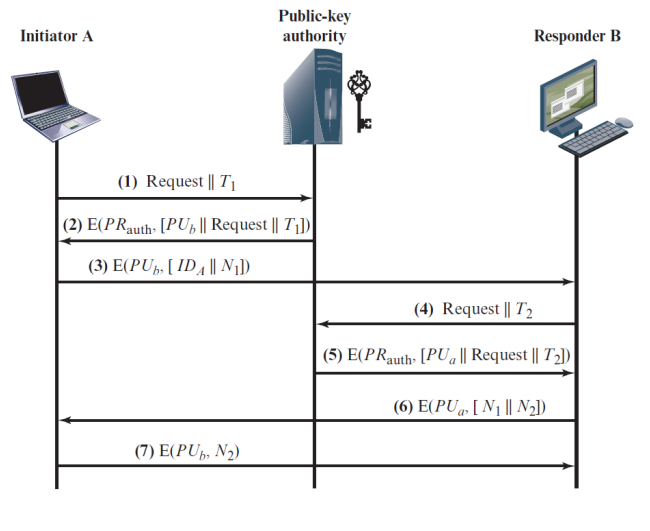
\includegraphics[width=1\textwidth]{images/chapter3/3-4.png}
    \caption{Scambio semplice.}
    \label{fig:3-4}
\end{figure}

Il certificato può essere ottenuto dalla Certification Autority o dall'utente.

\subsection{Certificati X.509}

Parte della serie X.500 che definisce un servizio di directory. Una directory può essere un serve o un insieme di server che mantengono un DB con info sugli utenti. 
Lo standard X.509 definisce un framework per la fornitura di servizi di autenticazione dalle directory dell'X.500 agli utenti (raccomanda RSA, non specifica l'algoritmo di hash da usare).

Uso del certificato:
\begin{itemize}
    \item Il certificato è "formato" da due parti: il certificato vero e proprio e il certificato firmato;
	\item Il certificato firmato non è altro che l'hash del certificato firmato con la chiave privata della CA;
	\item Un utente che vuole verificare il certificato passa all'algoritmo di verifica l'hash del certificato, il certificato firmato e la chiave pubblica della CA.
\end{itemize}

Un certificato si compone di:
\begin{itemize}
    \item Versione del certificato;
	\item Numero seriale del certificato all'interno della CA che l'ha rilasciato;
	\item Identificatore dell'algoritmo usato per la firma;
	\item Nome della CA;
	\item Periodo di validità:
	\item Nome dell'utente;
	\item Info culla chiave pubblica dell'utente;
	\item ID unico della CA;
	\item ID unico dell'utente;
	\item Estensioni;
	\item Firma (certificato firmato).
\end{itemize}

I certificati generati da una CA hanno le seguenti caratteristiche:
\begin{itemize}
    \item Ogni utente che ha accesso alla chiave pubblica della CA può verificare la chiave pubblica di un altro utente firmata dalla CA;
	\item Nessuno, eccetto la CA, può modificare un certificato senza essere individuato.
	\item Poiché i certificato non possono essere forgati, la directory in cui sono piazzati non richiede troppa sicurezza;
	\item Una volta che B è in possesso del certificato di A, sa che i messaggi cifrati con la chiave pubblica di A saranno al sicuro da intercettazione e che i messaggi firmati con la chiave privata di A saranno inforgiabili.
\end{itemize}

Catena di certificati: A vuole verificare il certificato di B, ma non conosce la chiave pubblica della CA di B. Se le due CA si sono scambiate le proprie chiavi (si sono certificate tra loro), A la può recuperare dalla directory della sua CA. In caso contrario, a partire dalle CA con cui la CA di A si è scambiata le chiavi, si procede a cercare la prima coppia di CA (una parente di A e una di B) che si sono certificate tra loro. Si costruisce quindi una catena di certificati. La catena ha la forma di un albero. Se un nodo, quindi CA, viene compromesso, allora anche il sottoalbero figlio viene considerato compromesso.

Revoca del certificato:
\begin{itemize}
    \item Ogni certificato contiene un periodo di validità, che solitamente viene sostituito prima della scadenza;
	\item Generalmente si tende a revocare un certificato prima della scadenza se:
	\begin{itemize}
	    \item La chiave privata dall'utente è compromessa;
		\item L'utente non è più certificato dalla CA;
		\item La CA è compromessa.
	\end{itemize}
	\item Ogni CA deve mantenere e rendere accessibile una lista dei certificati revocati non per scadenza.
\end{itemize}

\subsection{Certificati X.509 V3}

Include la possibilità di specificare estensioni (piuttosto che continuare ad aggiungere nuovi campi). Le estensioni possono riguardare:
\begin{enumerate}
    \item Info sulla chiave o sulla policy: copre info addizionali sull'utente e la CA, più indicatori sulle policy del certificato. Una policy sul certificato è un insieme nominato di regole che indica l'applicabilità del certificato a particolari comunità o classi di applicazioni con requisiti di sicurezza comuni. Contiene:
	\begin{itemize}
	    \item ID della chiave della CA;
		\item ID della chiave dell'utente;
		\item Uso della chiave (firma digitale, ripudio, crittografia delle chiavi, ecc.);
		\item Periodo di utilizzo della chiave privata;
		\item Policy del certificato;
		\item Mapping delle policy (consente a una CA di indicare altre CA equivalenti).
	\end{itemize}
		
	\item Attributi sulla CA o sull'utente: supportano nomi alternativi, in formati alternativi, per un soggetto del certificato o un emittente del certificato. Può contenere informazioni aggiuntive sul soggetto del certificato per aumentare la fiducia dell'utente del certificato che il soggetto del certificato sia una determinata persona o entità. I campi dell'estensione comprendono:
	\begin{itemize}
	    \item Nome alternativo del soggetto;
		\item Nome alternativo dell'emittente;
		\item Attributi sulla directory del soggetto.
	\end{itemize}
		
	\item Vincoli sul certificato: permettono di includere le specifiche di vincolo nei certificati emessi per CA da altre CA. I vincoli possono restringere le tipologie di certificati che possono essere emessi dalla CA soggetto o che possono verificarsi successivamente in una catena di certificazione. I campi sono:
	\begin{itemize}
	    \item Vincoli di base;
		\item Vincoli sui nomi;
		\item Vincoli sulle policy
	\end{itemize}
\end{enumerate}

Ogni estensione contiene: ID dell'estensione, indicatore di criticità, valore dell'estensione.

\subsection{Possibile scenario}
La RA ha il compito di raccogliere info su Bob per assicurarsi che sia chi dica di essere (\ref{fig:3-5}).

\begin{figure}
    \centering
    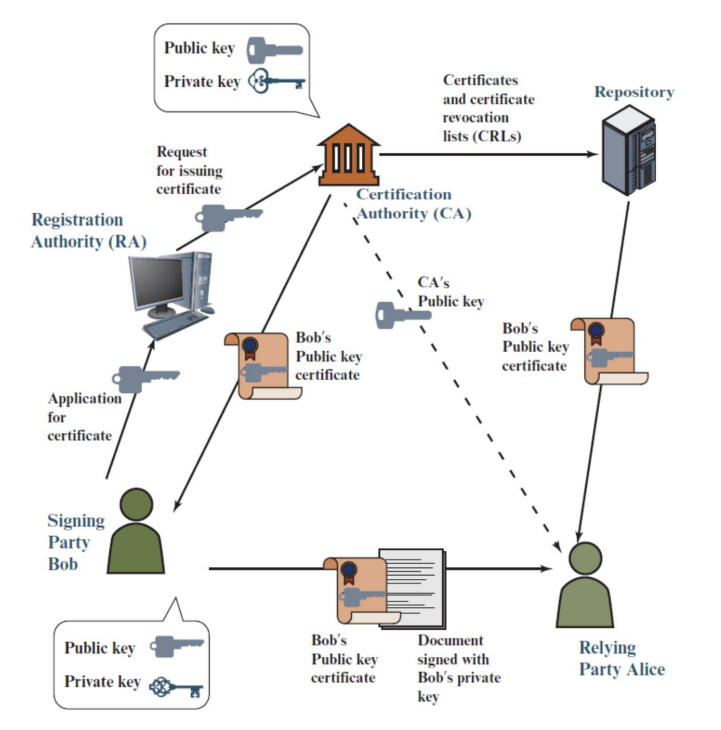
\includegraphics[width=1\textwidth]{images/chapter3/3-5.png}
    \caption{Scambio semplice.}
    \label{fig:3-5}
\end{figure}